\section{Introduction}

%\paragraph*{Brief introduction of your general area of interest: provide the \textbf{context} to the overall general setting.} 
\textit{Conformance checking} is an integral part of \textsc{Artificial Intelligence} {bridging} data mining and business process management \cite{bpm21}. It assesses whether a sequence of distinguishable events (i.e., a \textit{trace}) conforms to the expected process behaviour represented as a \textit{process model} \cite{RozinatA08}. When multiple distinct traces are considered in a log, model checking lists the set of traces satisfying the model \cite{BurattinMS16}. Models are composed of multiple human readable \textit{clauses} that should be  jointly satisfied (i.e., \textit{conjunctive query}) \cite{Li2020}; each of these is the instantiation of a specific behavioural pattern (i.e., \textit{template}) with specific data and action conditions. These high level representations can be also expressed as Finite State Machines \cite{MultiPerspective}. %Such a model might be either represented as a set of temporal clauses, determining correlations between events happening at a previous time of the trace (\textit{activation}) and others happening in the immediate future (\textit{target}).
{Despite the two approaches are equivalent}  \cite{AgostinelliBFMM21}, {the latter is rather inefficient for conformance checking traces with data payloads} \cite{bpm21}. %Declarative temporal rules are not limited to the mere presence of specific events within the trace, but also determine \RevRepl{how such clauses might occur}{temporal occurrence patterns}. 
{Declarative models are usually   the core} of AI's temporal decision making: by extracting a declarative model out of a hospital log \cite{mining} containing `successful' traces (e.g., correct procedures, adequate medication), we extract the temporal correlation conditions linking good pre-conditions to expected outcomes  \cite{Amantea2020}. An AI could then exploit such a model
for predicting which novel clinical situations represented as %on the novel hospital 
traces are likely to adhere to the expected clinical standards.
% \RevRepl{this}{the resulting mined} model \RevRepl{for a current trace to provide the action}{for determining} which \RevAdd{clinical situation} is likely to \RevRepl{be  the next correct decision}{adhere to the expected clinical standards}.

\begin{figure}
	\centering
	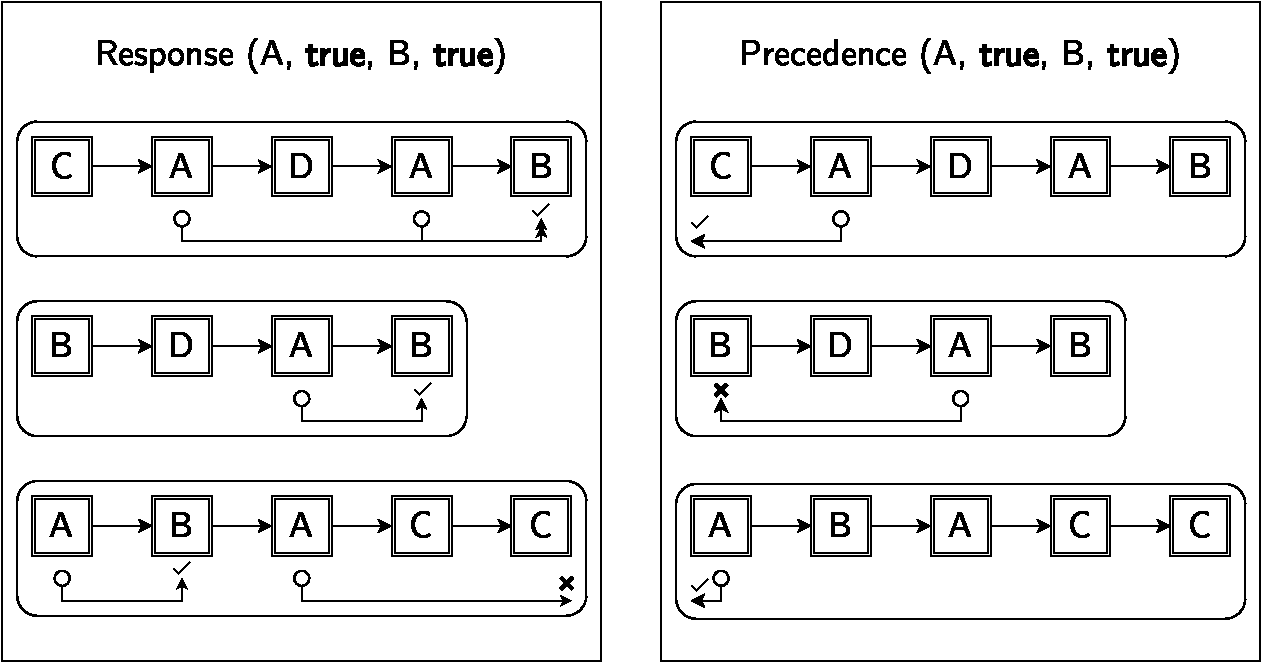
\includegraphics[width=.7\textwidth]{images/ActivationTargetExample.pdf}
	\caption{Two exemplifying clauses distinguishing \textsf{Response} and \textsf{Precedence} behaviours. Traces are represented as temporally ordered events associated to activity labels (boxed). Activation  (or target) conditions are here circled (or ticked/crossed). Ticks (or crosses) indicate a (un)successful match of a target condition. For all activations there must be an un-failing target condition; for precedence, we shall consider at most one activation (\S\ref{sec:DAD}). These conditions require the usage of multiple join tests per trace.}\label{fig:comparison}
\end{figure}
%\pdfcomment[author=Giacomo]{Please link this description to the infographics, that is going to describe the whole KnoBAB pipeline}
When a trace does not adhere to the model, we say that the trace is \textit{deviant} \cite{bpm21}. %\RevDel{In the case of traces, the order of the events is important, and temporal information of each event must be stored.}
E.g., Given a Declare template \textsf{Response}, \DeclareClause{Response}{A}{\textbf{true}}{B}{\textbf{true}} is the instantiated Declare \textit{clause} for \textit{activity labels} \texttt{A} and \texttt{B} stating ``\emph{If event \texttt{A}  happens, event \texttt{B}  must happen either contemporarily or anytime in the future}'' (\figurename~\ref{fig:comparison}); \texttt{A}  (\texttt{B}) is called  \textit{activation} (\textit{target}) condition; a trace would be a deviant \emph{iff.} a trace contained an instance of \texttt{A}  that was not followed by an instance of \texttt{B}. In \figurename~\ref{fig:comparison}, the last trace is the only deviant one. Furthermore, \textbf{true} predicates associated to activation (target) conditions can be enriched to express data conditions (\S\ref{sec:DAD}). As any declarative language, the specification of such templates can be expressed as expressions of logical operators: in this field, Finite Liniear Time Logic (\LTLf) is usually exploited. For instance, clause $\DeclareClause{Precedence}{A}{p}{B}{q}$ becomes $\WeakUntil{\neg(\texttt{B} \wedge q)}{(\texttt{A} \wedge p)}$, %\pdfcomment[author=Giacomo]{Please link this description to the infographics, that is going to describe the whole KnoBAB pipeline} 
where the binary operator $\WeakUntil{}{}$ denotes that either left-hand-side should always occur until the right- one is found for the first time in the trace, or the left-hand-side should always occur (\figurename~\ref{fig:comparison}). %Activation and target 
Conditions might %be 
also include % extended with 
\textit{correlation} conditions, thus expressing $\Theta$-joins between activated and targeted events. %only between their associated payload. 
This is a restriction over traditional relational algebra operators, as we are only interested in analysing such correspondence. %Figure \ref{fig:comparison} exemplifies such intuition.
%%{\color{red}[TODO: replace] To further decompose these clauses, algebraic notation can be used to represent the set of operators that are the constituents of a given clause. Declare templates can be represented using \LTLf \cite{Li2020}. This allows for a flexible conformance checking implementation, as each clause can be represented as a unique pairing of \LTLf operators and join operators, for insatnce $\mathbf{RespondedExistence(A,B)}$ becomes $\Future(A) \Rightarrow \Future(B)$\PopUpComment{Giacomo}{Please observe that mathcal should be used only by surrounding the symbol of interest. Otherwise, in some other scenarios, you might have faults. Still, we are going to use a box/diamond notation for this paper. I added some macros for that}. As part of the process mining pipeline, conformance checking is used to identify patterns emerging from a given log. Therefore, process mining can actually be reduced to a conformance checking problem.}\PopUpComment{Giacomo}{Some of the contents in here are good, and should be put elsewhere in the introduction. "In fact, despite these operators might be applied to query plans similarly to relational algebra operators, no work -- to the best of our knowledge -- exploited this possibility". But, this should be linked to another kind of problem, too!}



%\paragraph*{Why do I want to talk about this problem? Why is it relevant?} \textit{Because current literature is lacking of a given aspect} 
%\section{Motivating Example}\label{sec:mot}
%Correlations might be also exploited in 
Real business use case scenarios usually require such correlations. In a goods brokerage scenario \cite{PetermannJMR14},  items are traded between producers (vendors) and retailers (customers): each transaction starts with a vendor sending a sales quotation to a customer. If an offer is accepted and the order is confirmed, then the item is scheduled for delivery. When ready, a logistic operator collects it. %The 
%sales invoice and the sales order is then sent to the retailer. Next, both the producers and the retailers might rank the items on a scale from 0 to 10, where 0 denotes a despicable product while 10 denotes an excellent one. A retailer ranking a product extremely low can file a complaint ticket to the brokerage company which might grant a refund.
In this scenario, deviant traces are %traces that 
either do not reflect the company's rules or %traces that 
will potentially lead to retailers' complaints. %In particular, a company must send a product only after receiving the offer's acceptance. \dfrac{num}{den}
E.g., % business rule explicitly requiring correlations is the following:   
a late delivery complaint can occur only if the date the product is received is greater than the agreed time to receive it as registered in a previous agreement event. This situation cannot be directly expressed as a temporal pattern, as we also need to test the timestamps associated in the data payload. %Albeit this task requires to represent temporal information within the data perspective \cite{MultiPerspective}, this would require to express \textit{correlation} conditions (\S\ref{sec:DAD}) within the single Declare template of interest. 


%\paragraph*{Who might be interested in our solution? How these people might use this work?} \textit{Please provide the pieces of information that are specific to your own research field, and provide some use case examples motivating the practicality of your approach}  

{Conformance checking can be applied to several other non-business domains.} 
 \textit{First}, given that process model information can be exploited to represent 
  tasks performed by both physical and cybernetic agents \cite{Ioanna}, %this information can be exploited to detect
   \textbf{cyber-security attacks} can be detected through a model extracted from previous historical data, where specific attacks of interests are selected \cite{BENASHER201551,LagraaS20}. Then, the conformity of any trace to the model might be exploited for determining whether an attack occurred or not. \textit{Second}, \RevRepl{Mining particular patterns within this data }{temporal models extracted from} hospital logs, consisting of diagnoses and treatments with their respective outcomes, could aid \textbf{healthcare} professionals in \RevDel{future} \textbf{decision making} \cite{Amantea2020}. Such models enable explainable AI by associating a precondition to a consequence within a  clinical event of interest \cite{mining,KusumaKMHGJ20}. Conformance checking tools might then assess whether the specific clinical case abides to the declarative rules in the mined model, thus allowing the prediction of a specific clinical event of interest. \textit{Last}, most recent \textbf{video-games}  exploit AI features \cite{LiGT21}: existing state of the art exploits automata \cite{Miyake2017} for modelling \textsc{Non Player Character}'s behaviours. As Declarative models and automata are completely equivalent approaches, developers might exploit the former to  compactly represent the latter. Furthermore, as debugging AI in video-games is a crucial challenge \cite{john2019debugging}, conformance checking solutions might be exploited for debugging unexpected behaviours. As AAA videogames already  track and log both players and NPC actions\footnote{\url{https://battlefieldtracker.com/}}, it might be also possible to use game logs for distinguishing winning strategies from losing ones \cite{mining}. As a result, analysis of an ongoing trace at runtime might `suggest'  actions beneficial to the player based on the game state.%, with the current strategy they are pursuing.

%\begin{itemize}
%	%\item A cyber-security attack, where a model can be extracted from previous invasions allowing common patterns to be identified. Some solutions such as \cite{BENASHER201551} use technologies to identify this, but they do not use conformance checking. 
%	\item A hospital log \cite{Amantea2020} [\dots]  \MarkText{In addition to the process discovery, these approaches are `opening the way to perform conformance checking and enhancement', which further justifies our argument that a process mining technique can be reduced to a conformance checking problem.} \PopUpComment{Giacomo}{The problem with this is that it does not explain how this could be done. We shall discuss this in person. Please see the above rephrasing.}
%	%\item Suggesting actions to players in video games. Conformance checking applications for AI in video games has not previously been research; existing state of the art \cite{Miyake2017} use either automata or machine learning. Process mining would allow models to be extracted that represent unique strategies players have attempted in the past. Information regarding their `success' can also be stored. As a result, analysis of an ongoing trace at runtime would then allow the model to `suggest' an action that is beneficial to the player based on the current state of the game, with the current strategy they are pursuing.
%\end{itemize}




\iffalse
%\paragraph*{What do I want to say (to the research community), precisely.} \textit{I want to communicate the general problem that I am aiming to solve} 
Current state of the art conformance checking solutions do not exploit the benefits of storing data in a custom relational database. When running queries, the same data is often accessed multiple times \cite{BurattinMS16,bpm21}. This is especially the case in the process of data-mining with large workloads \cite{SchonigRCJM16}, where the identification of patterns often share similar subqueries. On the other hand, Existing solutions \RevDel{, such as} \cite{BellatrecheKB21}\RevDel{, exploit this by} identify\RevDel{ing} \RevRepl{the}{common} sub\RevAdd{-}expressions within \RevRepl{a query}{several queries running contemporarely}\RevDel{ occurring more than once}, therefore \RevRepl{requiring only one computation}{reduce both the data access and the computation overhead to a minimum.} \RevAdd{This can be easily relate to the conformance checking problem, where multiple declarative clauses from the same model might be assessed contemporarily}. By decomposing these queries into \LTLf, a similar approach can also be followed. We propose that the queries, decomposed into \LTLf operators, can also follow a query plan similar to \cite{BellatrecheKB21}. We extend the approach by adapting the query plan to \RevRepl{use relational algebra with}{express \LTLf operators similarly to relational algebra operations}, where common sub-expressions can still be rationalised. Still, there is some prior work on \RevDel{Another approach proposes a solution that} decompos\RevRepl{es}{ing} clauses into traditional SQL queries \cite{SchonigRCJM16}. This solution \emph{does} exploits the benefits of using a relational database (and therefore query plans) by transforming declare clauses into traditional SQL queries. However, this solution is limited as it \RevRepl{does not}{neither} consider\RevAdd{s} data conditions (only event identifiers), \RevAdd{nor considers multiple clauses pertaining to disparate Declare templates}. This provides less functionality than we propose, where we are data-aware and theta conditions can be taken into account when performing any operators.



%Last, we can observe that some temporal information cannot be expressed by data-agnostic Declare templates. For example, a late delivery complaints occur if the date of a product is greater than the agreed time to deliver it in the previous sales order. This situation cannot be directly expressed as a $\textsf{Precedence}$, as we also need to test the timestamps as both data and event timestamps. Albeit this task requires to represent temporal information within the data perspective \cite{MultiPerspective}, this would require to express \textit{correlation} conditions (see \S\ref{ssec:dad}) within the single Declare template of interest. In the present work, we discard the possibility of expressing such correlation constraints: please observe that this is a quite common consideration within the spectrum of Business Process Management, and therefore we will continue to work under this working assumption \cite{10.1007/978-3-642-40176-3_8}. Nevertheless, we are planning to extend the proposed approach so to perform conformance checking containing correlation constraints. 
%Conformance checking is an integral part of artificial intelligence that bridges data mining and business process management. 


%Conformance checking can be extremely computationally intensive, both in time and storage, so optimised solutions are necessary to ensure a well performant implementation. To our knowledge, no solution existing whereby a relational base exploits optimised query plans, adapting solutions such as \cite{BellatrecheKB21}, in a business process environment using LTLf.
\medskip


\paragraph*{Now, communicate our idea also to the people working in our same area!} \textit{In particular, this means that we can go down in technicalities on what we want to solve, which are the primarily goals of our research, and which are the intermediate requirements/results leading to the results that we expect.} 
Assessing the ability of each trace to satisfy a given temporal logical constraint is computationally costly: intuitively, checking whether a \textsf{Response} condition is met in a trace will require the possibility of tagging those with event distinctive labels, and to evaluate if the condition holds by joining each possible event A in the temporal series with the B events happening in the future, if any, and counting if all of the A events within the series satisfy such criteria. As we might see, this might become quite costly in big data scenarios, where both traces' lengths and their number is considerable high. If we want to also list all of the traces satisfying this condition, this computational burden is worsened by the costly \texttt{Group By} operation on traditional data bases, thus including document-oriented ones \cite{THoSP}.

As process mining can be reduced to a conformance checking problem, a given log can be queried against a declarative model at runtime, and the same conformance checking calculations can be applied to generate its conformance \emph{at the current time}. Therefore, KnoBAB provides an optimized representation of the trace logs over which the declarative models $\mathcal{M}$ are going to be both queried and mined with \LTLf.

We propose a knowledge base, KnoBAB, which provides efficient conformance checking by adapting query plan optimisations \cite{BellatrecheKB21} to \LTLf. In addition, we provide data-aware capabilities, which discussed database solutions do not. KnoBAB provides the conformance of a \emph{trace} to a set of clauses, not the conformance of a clause against a log. This is more valuable in scenarios where trace information could point to where, and why, it was a deviant. Such knowledge could then be used for many features, such as generating the repair for this trace.
\medskip


The greatest amount of performance gain is due to the custom query plan, structured in such a way that multiple queries are stored within a graph, and then batch jobs are run using \textbf{parallelisation}. When process mining, large numbers of queries are performed, therefore there will be many instances of duplicate data accessing, resulting in poor optimisation. In this approach, there is the guarantee that unique data elements are obtained and processed only once, while current state of the art process-mining approaches access data per query. 
\fi

Although there are solutions representing a set of model clauses as SQL queries \cite{Schonig15,SchonigRCJM16}, these neither evaluate the satisfiability for every single trace, nor return the traces that satisfy them, but only associate support and confidence values to each of said clauses. However, in this paper, we show that these queries can be extended so as not only to evaluate satisfiability per trace but also by returning the set of traces that satisfy every single clause, thus adhering to the definition from conformance checking literature (\S\ref{sec:DAD}). In doing so,  we are forced to introduce  aggregation and nesting operations, which are not generally efficient. This fact is supported by experimental evidence (\S\ref{ssec:sqlmin}), where we also extend the relational representation of traces from \cite{Schonig15,SchonigRCJM16} (\S\ref{ssec:dl}). Our specific contribution is then the provision of specific operators (\xLTLf) implementing the \LTLf operators over the relational database model and tailored for solving the conformance checking in Declare (\S\ref{sec:xltlf}), and the optimization of the query plan as proposed by \cite{BellatrecheKB21} (\S\ref{ssec:xltlf}): this proves to be more efficient than any solution relying solely on the SQL language. Our proposed solution is then implemented in KnoBAB\footnote{[URL REMOVED FOR DOUBLE BLIND REVIEW].}

Even state-of-the-art implementations, explicitly engineered to solve the conformance checking problem without relying on a 
relational representation of traces, are not particularly efficient \cite{BurattinMS16}. This solution, not being able to assemble the previously described \LTLf operators within a query plan, can neither minimize the access operations to the trace data nor  minimize the re-computation of sub-expressions that appear frequently in the model as recently proposed by \cite{BellatrecheKB21}. Further experimental shreds of evidence support such theoretical claims (\S\ref{ssec:declan}): in the first instance, these show that our solution is already more efficient than the state of the art in the literature by two orders of magnitude (hundredths of a second vs. seconds). Furthermore, by using different Declare models composed of several clauses accessing the same activation and target conditions, except the data correlations, our solution preserves a constant running time with fewer temporal fluctuations, while the running time from  \cite{BurattinMS16} is directly proportional to the size of the model.

\begin{sidewaysfigure}
	\centering
	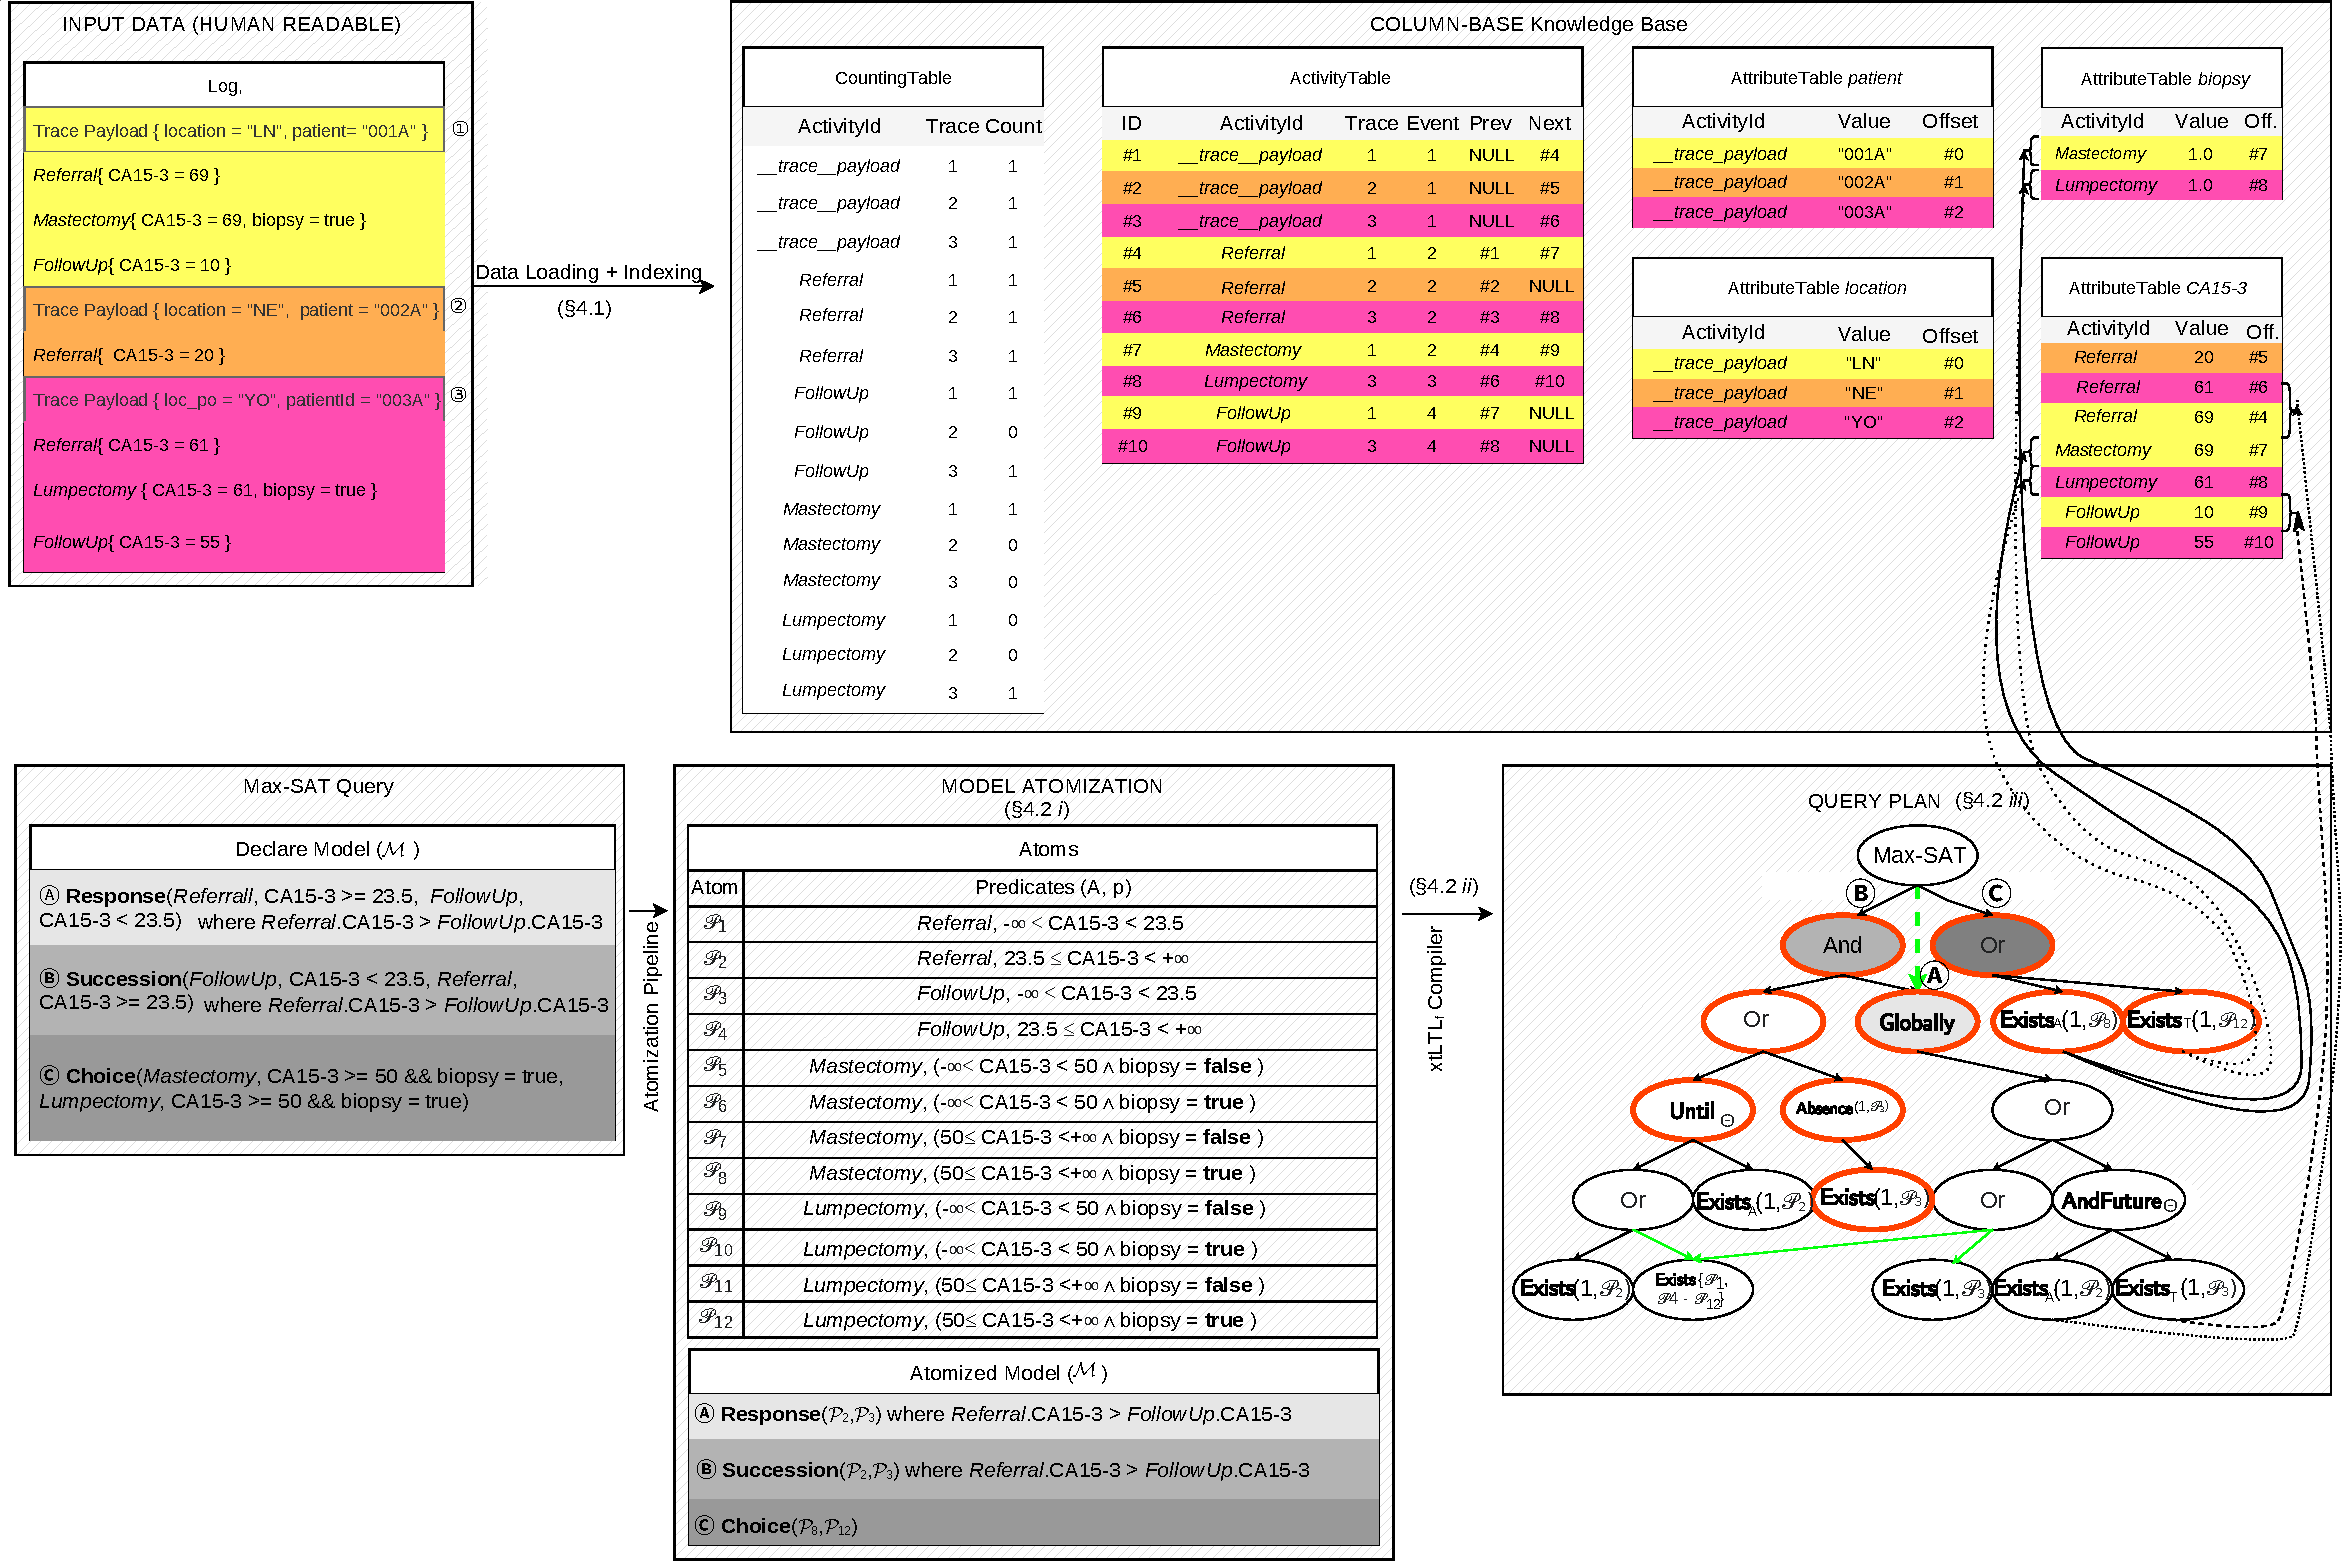
\includegraphics[width=\textwidth]{images/knobab_pipeline.pdf}
	\caption{KnoBAB architecture for data loading and querying for a bank management system. Events (A,B,C) are contained within $\mathcal{L}$. Events are ordered top-down, and traces are represented with unique colouring. } \label{fig:knobab_pipeline}
\end{sidewaysfigure}

In addition to the aforementioned major contributions and in order to achieve the introduced results, we also provide these ancillary contributions: as demonstrated by \figurename~\ref{fig:knobab_pipeline}, we show how to extend the relational solution for representing logs from \cite{Schonig15,SchonigRCJM16} with a counting table and a column-based relational model for representing data payloads associated to each event and trace (\S\ref{ssec:dl}). Second, we design a query compiler (\S\ref{sec:qc}) transforming each Declare model composed of multiple single clauses into a DAG query plan. Next, we designed an execution engine running the \xLTLf operators either sequentially or in parallel (\S\ref{ssec:xltlf}).